\documentclass[a4paper,12pt]{UoBnote}

\usepackage{enumitem}
\usepackage{listings}
\usepackage{color}
\usepackage{graphicx}
\usepackage{float}

\floatplacement{figure}{H}

\lstset{language=sh}
\setlength{\parskip}{1em}
\author{Mike Knee}

\shorttitle{Numerical Modelling}
\title{Worksheet 1 Report}
\date{\today}
\issue{1}

\begin{document}

\maketitle
\tableofcontents
\vspace{1cm}\hrule \vspace{1cm}

\section{Question 1}

For the first excercise a number of commands were input to the linux bash prompt, in order to understand what the different commands do and how to use them. Thecommands are listed here in order, with the output following and finally a description of what the command has done.
\begin{enumerate}[label=\alph*)]
	\item mkdir compphys

		No output, but a new directory has been created called ``compphys''
	\item cd compphys

		No output again, but now the current working directory is ``~/compphys''
	\item cat $>$ file1.txt [rtn] this is my first file [rtn][ctrl-c]

		No output is printed to the screen, however a new file called ``file1.txt'' has been created, containing the text ``this is my first file''
	\item ls

		Ouput is: 
		\begin{verbatim}
		file1.txt
		\end{verbatim}

		The ls command lists the contents of the current working directory.
	\item more file1.txt

		Output is:
		\begin{verbatim}
		this is my first file
		\end{verbatim}

		The more command pages files to the standard output, seen as the file ``file1.txt'' only has one line, that line is simply printed to the terminal.
	\item xclock\&

		Output is shown in figure \ref{fig:xclock}.
		\begin{figure}
			\centering
			
\includegraphics{xclock}
			\caption{xclock open through the ssh session}
			\label{fig:xclock}
		\end{figure}

		The xclock\& command starts an xclock process. This will be opened on the client side through ssh if X11 forwarding is enabled, and the client is able to display xwindow objects. The ampersand is to tell the process to start the process in the background, ie. to allow the shell session to continue while xclock is still running.
	\item whoami

		Output is:
		\begin{verbatim}
		mfk364
		\end{verbatim}

		This command prints the username of the current user.

	\item man ls

		Output is a man page, a text document describing the usage of the ``ls'' command. Calling man $<$command$>$ will display a man page on any command with proper documentation. Figure \ref{fig:manpage} shows the top of the ls man page.
		\begin{figure}
			\centering
			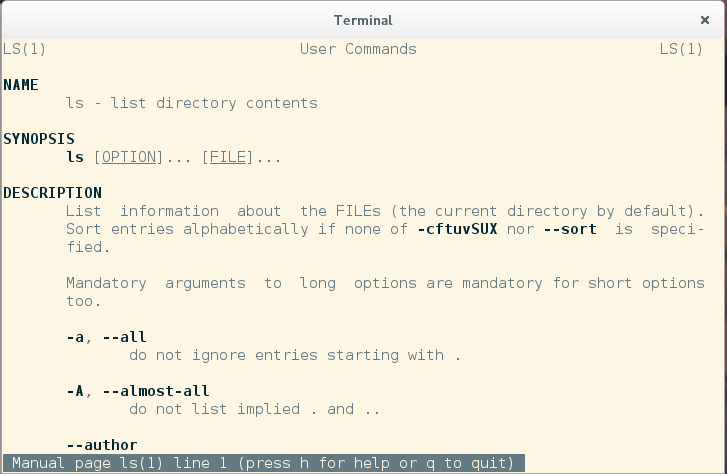
\includegraphics[scale=0.3]{manls}
			\caption{Top of the man page for the ``ls'' command}
			\label{fig:manpage}
		\end{figure}

	\item top

		Output is a display of running processes, ordered by CPU usage. The column processes are sorted by, and other options can be changed using commands while top is running. Figure \ref{fig:top} shows top while running, with the columns sorted by CPU usage.
		\begin{figure}
			\centering
			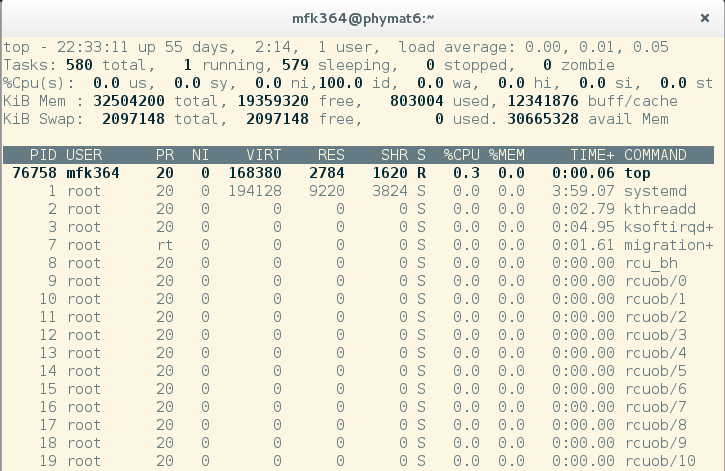
\includegraphics[scale=0.3]{top}
			\caption{The ``top'' command in action}
			\label{fig:top}
		\end{figure}

	\item kill

		The ``kill'' command is used to stop running processes. In order to use kill one needs the PID of the process to be stopped. For this the ``ps'' command is used, which lists all the processes running under the current user's UID. Once a PID is known ``kill [PID]'' will send a terminate signal to the process.

		The output of the kill command is:
		\begin{verbatim}
		[running processes] Terminated\tab [process name]
		\end{verbatim}

	\item ps -u [username]

		As described above the ``ps'' command displays currently running processes. The -u option denotes that all the processes belonging to a user specified by [username] should be displayed. The default behaviour of ``ps'' is to display the processes belonging to the current user running in the current TTY. 

		An example output of the ``ps -u [username]'' is shown in figure \ref{fig:ps}. 
		\begin{figure}
			\centering
			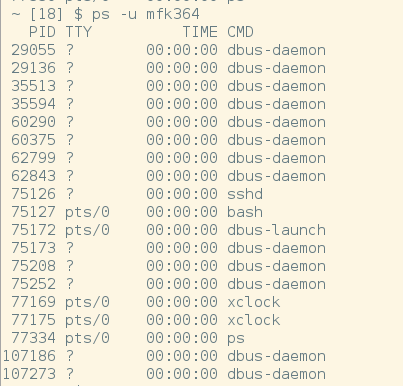
\includegraphics[scale=0.3]{ps}
			\caption{An example of ``ps -u [username]'' output}
			\label{fig:ps}
		\end{figure}

\end{enumerate}

\section{Question 4}


For this question a C++ program was required to calculate different powers of $\phi$ (the silver ratio), given by $\phi = \frac{-1 + \sqrt{5}}{2}$, and output the data to a file. The source code for this program is called ``w1q4.cpp'', and when run will output data to a file called ``output''. The code calculates and writes the power of phi by basic multiplication in lines 53-56.

SHOW HERE...

The function recursion\_relation (starting at line $20$ in the code) is the reursive function that uses the recursion relation defined as $\phi^{n+1}=\phi^{n-1}-\phi^{n}$. When the programme is run with values of $N$ greater than around $40$ the programme runs extremely slowly. This is because this recursive function runs in $O(n^2)$ time, and is therefore very slow.



\end{document}

